\documentclass[11pt]{article}
\usepackage[utf8]{inputenc}
\usepackage[T1]{fontenc}
\usepackage{geometry}
\usepackage{graphicx}
\usepackage[francais]{babel}


\title{TDDC32 - Ray Tracing Engine}
\author{Simon Vernhes \texttt{<simon@vernhes.eu>}}
\date{} 

\begin{document}

\maketitle  
\section{Introduction}
This project consist in programming a Ray Tracer (graphic renderer tool). A Raytracer compute pixel by pixel the image to render using a description of the scene.

The final program should take a textual description of a scene, and render the corresponding image.

\section{Modules}
We can easily identify 3 modules for this program as show in the figure below : the parser, the world model, the renderer.

\begin{figure}[ht]
  \centering
  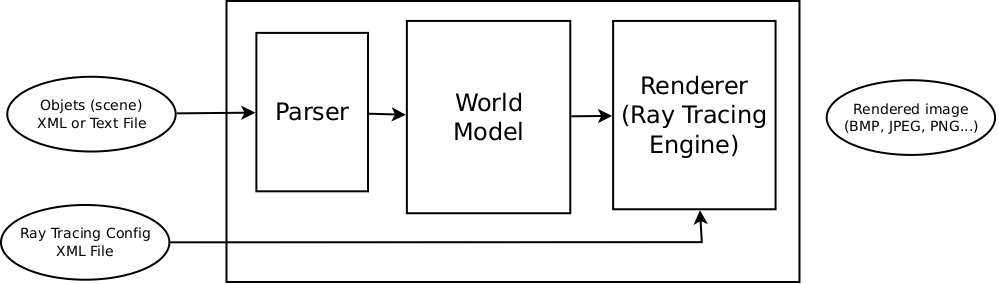
\includegraphics[height=5cm]{Diagramme1.png}
  \caption{Software flow}
\end{figure}

\section{Iterate and Increment}
The iterate and increment principle will be widely used in this project. So a basic raytracer will be create first : only a few object to represent the scene (sphere, cube, plan), only color instead of real texture...
Then we can add more functionalities, more object etc... 

\end{document}

